\documentclass[conference]{IEEEtran}
\IEEEoverridecommandlockouts
\usepackage{cite}
\usepackage{amsmath,amssymb,amsfonts}
\usepackage{algorithmic}
\usepackage{graphicx}
\usepackage{textcomp}
\usepackage{xcolor}
\usepackage{booktabs}
\usepackage{microtype}
\usepackage{tabularx}
\usepackage{tikz}
\usetikzlibrary{arrows.meta,positioning,fit,backgrounds}
\renewcommand{\IEEEkeywordsname}{Keywords}

\def\BibTeX{{\rm B\kern-.05em{\sc i\kern-.025em b}\kern-.08em
    T\kern-.1667em\lower.7ex\hbox{E}\kern-.125emX}}

\begin{document}

\title{BioLearnX: A Self-Improving Multi-Agent Framework for Personalized Biology Learning through Interactive Visualization, Adaptive Assessment, and Multilingual Content Generation}

\author{
\IEEEauthorblockN{Kojithan P. Y.\IEEEauthorrefmark{1}, Baskaran V.\IEEEauthorrefmark{1}, Nishara T.\IEEEauthorrefmark{1}, Sarmitha S.\IEEEauthorrefmark{1}, Nuwan Kodagoda\IEEEauthorrefmark{2}, Malithi Nawarathne\IEEEauthorrefmark{2}}
\IEEEauthorblockA{\textit{Faculty of Computing, Sri Lanka Institute of Information Technology, Malabe, Sri Lanka}\\
Email: \{\IEEEauthorrefmark{1}it22264220, \IEEEauthorrefmark{1}it22172600, \IEEEauthorrefmark{1}it22223876, \IEEEauthorrefmark{1}it22637482\}@my.sliit.lk, \{\IEEEauthorrefmark{2}nuwan.k, \IEEEauthorrefmark{2}malithi.n\}@sliit.lk}
}

\maketitle

\begin{abstract}
Biology learners typically move between separate tools for diagrams, revision, assessment, and note-taking, and few of these tools adapt to the individual learner or improve from experience. This paper presents BioLearnX, a multi-agent research framework that investigates whether four complementary agentic subsystems --- interactive visual generation, adaptive assessment, multilingual audio review, and handwritten-note recovery --- can share a common architectural pattern: retrieval-grounded large language model (LLM) agents, orchestrated as explicit graphs, that are evaluated by independent critics and improved only through validation-gated feedback. The visualization subsystem combines a catalog-driven anatomy specification extracted by an instruction model, image synthesis with a rectified-flow diffusion transformer, a dual CLIP/vision-language-model critic with a reflection-and-retry loop, segmentation-grounded interactive region explanation, and two-dimensional-to-3D asset conversion. The assessment subsystem generates curriculum-grounded, Bloom's-taxonomy-mapped questions from learner-uploaded documents and adapts difficulty from response history. The note-recovery subsystem applies fine-tuned super-resolution and optical character recognition models to enhance and transcribe low-quality Sinhala handwriting, with Tamil and English translation. The audio-review subsystem provides multilingual (Tamil, Sinhala, English, and code-mixed) spoken question answering grounded in the learner's own material. All four subsystems are implemented as independently deployable services on serverless GPU infrastructure and share a feedback-to-memory-to-skill-evolution lifecycle that gates every behavioral change behind held-out, paired evaluation. We describe the system design and the reproducible evaluation protocols implemented across the framework. An end-to-end baseline evaluation against the live deployment compares raw FLUX.1-dev output with our full visual pipeline (prompt enhancement under deployed persona/skill rules, FLUX.1-dev diffusion, and Qwen2.5-VL automatic structure labeling): the proposed pipeline achieves substantial gains in VLM visual alignment ($8.67 \pm 0.58$ vs.\ $6.00 \pm 3.46$, $+44.5\%$) and pedagogical usefulness ($7.67 \pm 0.58$ vs.\ $5.00 \pm 3.46$, $+53.4\%$), consistently producing 8 verified, callout-annotated anatomical structures per image versus 0 for the unlabeled baseline, while collapsing generation variance ($\sigma=0.58$ vs.\ $3.46$). We report these empirical findings alongside an architectural audit and pre-registered evaluation protocols for the full multi-agent ecosystem.
\end{abstract}

\begin{IEEEkeywords}
multi-agent systems, large language models, retrieval-augmented generation, parameter-efficient fine-tuning, text-to-image generation, optical character recognition, adaptive learning, biology education
\end{IEEEkeywords}

\section{Introduction}

Learning biology well requires moving fluidly between several representations of the same material: a labeled diagram of an organ system, a self-test that adapts to what the learner has already mastered, a spoken explanation for revision on the move, and usable notes recovered from a lecture photograph or a handwritten page. Commercial and open-source tools typically address one of these modes in isolation, and few of them adapt their own behavior from evidence of what worked for a given learner or a given class of requests. Two distinct problems are therefore left largely unaddressed by existing tools: (1) fragmentation across modalities --- visual, assessment, spoken, and written --- that a single learning session actually needs, and (2) the absence of a disciplined mechanism for an AI learning tool to improve itself without silently degrading correctness or safety.

Recent generative-AI research in anatomy and medical education has begun to explore embodied, conversational virtual assistants in immersive environments \cite{anatomyvr}, and separate lines of work have produced strong building blocks that make a more integrated approach practical: instruction-tuned and vision-language foundation models that can be adapted cheaply with low-rank fine-tuning \cite{lora,qlora}; promptable image segmentation that generalizes across domains \cite{sam2}; rectified-flow diffusion transformers capable of photorealistic, instruction-following image synthesis \cite{flux}; and agent frameworks --- reflection \cite{reflexion}, self-refinement \cite{selfrefine}, and explicit stateful orchestration graphs --- that let an LLM critique and retry its own output before it reaches a learner. What has not been demonstrated is a single research framework that applies these building blocks consistently across visualization, assessment, spoken review, and document recovery, under one shared, evidence-gated improvement lifecycle.

This paper presents \textbf{BioLearnX}, a four-subsystem research framework built to close that gap for biology education. Each subsystem is designed and implemented independently by one member of the project team, but all four share the same underlying principles: agentic pipelines orchestrated as explicit graphs rather than a single monolithic prompt; retrieval that grounds generation in the learner's own curriculum material; an explicit separation between raw user feedback (never trusted directly) and reviewed, evidence-backed memory or skill updates; and independent, automated critics that gate output quality before a result reaches the learner.

The contributions of this paper are:
\begin{enumerate}
\item A catalog-driven, LoRA-adapted \textbf{interactive biology visualization pipeline} that converts a natural-language learning request into a validated anatomical specification, a generated educational image, an independently critiqued and retried result, click-to-identify region explanations, and an optional 3D asset --- described in Section~\ref{sec:viz} and evaluated by the protocol in Section~\ref{sec:protocols}.
\item An \textbf{adaptive, curriculum-grounded assessment pipeline} that generates Bloom's-taxonomy-mapped questions from uploaded material and adapts difficulty and topic recommendations from response history --- described in Section~\ref{sec:quiz}.
\item A \textbf{fine-tuned super-resolution and OCR pipeline} for low-quality Sinhala handwriting, with Tamil/English translation, evaluated against a non-fine-tuned baseline using character error rate (CER), word error rate (WER), and exact-match accuracy --- described in Section~\ref{sec:ocr} and Section~\ref{sec:protocols}.
\item A \textbf{multilingual, retrieval-grounded spoken question-answering pipeline} (Tamil, Sinhala, English, and code-mixed) for conversational revision --- described in Section~\ref{sec:audio}.
\item A \textbf{shared, validation-gated feedback-to-skill-evolution lifecycle} used across the subsystems, in which a behavioral change is deployed only after paired, held-out evaluation shows a measured improvement over the currently deployed version --- described in Section~\ref{sec:lifecycle}.
\end{enumerate}

The remainder of this paper is organized as follows. Section~\ref{sec:related} reviews related work. Section~\ref{sec:arch} describes the shared system architecture and design patterns. Section~\ref{sec:methods} details the design and implementation of each subsystem. Section~\ref{sec:setup} defines the experimental setup already implemented for this study. Section~\ref{sec:results} reports results. Section~\ref{sec:discussion} discusses the findings. Section~\ref{sec:limitations} states limitations and threats to validity, and Section~\ref{sec:conclusion} concludes with future work.

\section{Related Work}
\label{sec:related}

\subsection{Diffusion-Based and Agentic Image Generation}

Rectified-flow diffusion transformers such as FLUX.1 \cite{flux} have made high-fidelity, instruction-following text-to-image generation practical at accessible parameter counts, but a single forward pass through such a model provides no guarantee that a generated image is factually or pedagogically correct. Agentic approaches address this by wrapping generation in a critique-and-retry loop: Reflexion \cite{reflexion} shows that an LLM agent that verbally reflects on a failed attempt and retries with that reflection as context outperforms agents that retry blindly, and Self-Refine \cite{selfrefine} shows the same model can act as its own critic without additional training. The visualization subsystem in this paper (Section~\ref{sec:viz}) applies this pattern with an explicit, \emph{independent} dual critic rather than self-critique, and separates the critic's role (scoring and diagnosis) from the retry mechanism (targeted regeneration).

\subsection{Vision-Language Grounding and Segmentation}

Interactive, click-to-identify explanation of an image region requires both precise segmentation and grounded semantic reasoning. SAM~2 \cite{sam2} extends promptable segmentation to produce high-quality masks from a point or box prompt without requiring the segmentation model to make any semantic claim about what it has segmented. Qwen2.5-VL \cite{qwen25vl} provides the complementary capability: native bounding-box localization and open-vocabulary visual question answering grounded in the pixels actually presented, which is the property this paper's interactive-region agent (Section~\ref{sec:viz}) depends on to avoid asserting the presence of a structure that is not visibly supported by the image.

\subsection{Parameter-Efficient Fine-Tuning}

Full fine-tuning of a multi-billion-parameter language model is impractical for a narrow, domain-specific task such as anatomical specification extraction or Sinhala handwriting recognition. Low-Rank Adaptation (LoRA) \cite{lora} freezes the pretrained weights and learns a small pair of low-rank update matrices per layer, and QLoRA \cite{qlora} extends this to 4-bit-quantized base models, making adapter training feasible on a single consumer or cloud GPU. This paper uses LoRA fine-tuning for the anatomy specification task (Section~\ref{sec:viz}) and fine-tunes encoder-decoder OCR and super-resolution models directly for the Sinhala-handwriting task (Section~\ref{sec:ocr}), evaluating both against their respective non-fine-tuned or pre-migration baselines rather than assuming a gain from fine-tuning alone.

\subsection{Retrieval-Augmented Generation and Agent Memory}

Grounding generation in a learner's own curriculum material requires efficient semantic retrieval. Sentence-BERT \cite{sbert} provides compact sentence embeddings suitable for similarity search at low latency, and Hierarchical Navigable Small World (HNSW) graphs \cite{hnsw} provide the approximate-nearest-neighbor index structure used to retrieve from a large embedding store in sublinear time. Beyond one-shot retrieval, an agent that is meant to improve over many sessions needs a policy for what evidence is durable enough to change its behavior; this paper's shared feedback lifecycle (Section~\ref{sec:lifecycle}) adopts the general pattern of separating raw interaction evidence from reviewed, promoted memory, gated by repeated, cross-session evidence before any prompt or rule is changed.

\subsection{Generative AI in Anatomy and Biology Education}

Prior work has begun to apply generative AI to anatomy education, including generative-AI-based conversational virtual assistants embedded in immersive virtual reality environments for anatomy question answering \cite{anatomyvr}. That line of work targets verbal, embodied interaction within a VR environment; it does not address on-demand generation of new, structurally validated 2D/3D visual content, nor does it combine visualization with adaptive assessment, multilingual spoken review, and handwritten-note recovery under one evaluation-gated improvement lifecycle. This is the gap BioLearnX addresses.

\section{System Overview and Shared Design}
\label{sec:arch}

BioLearnX is organized as a research monorepo of four subsystems that are developed, deployed, and --- at the current stage of the project --- evaluated \textbf{independently}, unified by a shared research vision and a common set of architectural patterns rather than a single production entry point (Fig.~\ref{fig:arch}). A unified interface and shared learner-profile layer across all four subsystems is explicitly future work (Section~\ref{sec:conclusion}), not a claim of this paper.

\begin{figure}[t]
\centering
\resizebox{\columnwidth}{!}{%
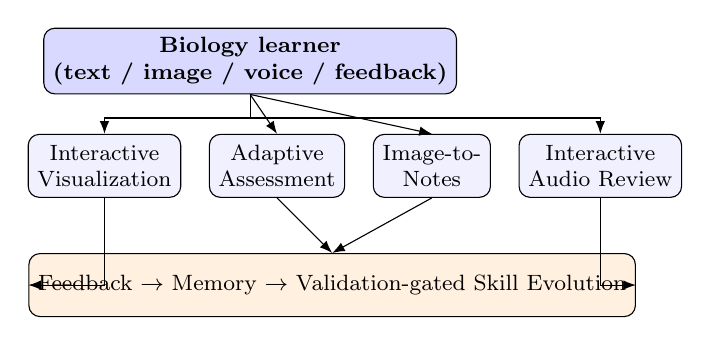
\begin{tikzpicture}[
  node distance=5mm and 3.5mm,
  box/.style={draw, rounded corners, align=center, minimum height=8mm, font=\footnotesize, fill=blue!6},
  learner/.style={draw, rounded corners, align=center, minimum height=8mm, font=\footnotesize\bfseries, fill=blue!15},
  shared/.style={draw, rounded corners, align=center, minimum height=8mm, font=\footnotesize, fill=orange!12},
  arrow/.style={-{Latex[length=1.6mm]}, thin}
]
\node[learner] (learner) {Biology learner\\(text / image / voice / feedback)};

\node[box, below=of learner, xshift=-1.85cm] (viz) {Interactive\\Visualization};
\node[box, right=of viz] (quiz) {Adaptive\\Assessment};
\node[box, right=of quiz] (notes) {Image-to-\\Notes};
\node[box, right=of notes] (audio) {Interactive\\Audio Review};

\node[shared, below=7mm of quiz, xshift=7mm, minimum width=6.2cm]
  (fb) {Feedback $\rightarrow$ Memory $\rightarrow$ Validation-gated Skill Evolution};

\draw[arrow] (learner.south) -- ++(0,-3mm) -| (viz.north);
\draw[arrow] (learner.south) -- (quiz.north);
\draw[arrow] (learner.south) -- (notes.north);
\draw[arrow] (learner.south) -- ++(0,-3mm) -| (audio.north);

\draw[arrow] (viz.south) |- (fb.west);
\draw[arrow] (quiz.south) -- (fb.north);
\draw[arrow] (notes.south) -- (fb.north);
\draw[arrow] (audio.south) |- (fb.east);
\end{tikzpicture}%
}
\caption{BioLearnX system overview. Four independently deployable subsystems share a common feedback-to-memory-to-skill-evolution lifecycle (Section~\ref{sec:lifecycle}); no unified runtime interface exists yet (Section~\ref{sec:limitations}).}
\label{fig:arch}
\end{figure}

\subsection{Agentic Orchestration}

Three of the four subsystems (visualization, assessment, audio review) implement their multi-step pipelines as explicit stateful graphs using LangGraph \cite{langgraph} rather than a single long prompt: each pipeline stage is a graph node that calls one independently deployed agent service over HTTP, receives a partial state update, and passes control to the next node. Errors are captured in pipeline state rather than raised, so a failure in one stage does not silently corrupt the state consumed by later stages. Every agent is deployed as an independent serverless function (Modal) behind a FastAPI REST endpoint, which keeps each subsystem's deploy lifecycle decoupled from the others and lets orchestration be tested against the same HTTP contract that any other client would use.

\subsection{Agent Context: Persona, Skill, and Memory}

Every agent in the visualization and audio-review subsystems is defined by three layers of context with different update policies: (1) a short, fixed \emph{persona} statement that is not subject to runtime modification; (2) a \emph{skill} document (\texttt{SKILL.md}) that encodes task-specific operating procedure and can only be changed through an evidence-gated evolution process (Section~\ref{sec:lifecycle}); and (3) a \emph{memory} layer of durable, reviewed lessons retrieved at request time. This separation keeps safety-relevant behavior outside of any component that learns from feedback.

\subsection{Feedback-to-Skill-Evolution Lifecycle}
\label{sec:lifecycle}

A learner's like or dislike on a given output is stored against the specific agent that produced it. A dislike triggers a targeted retry by that agent alone, without discarding correct upstream work from earlier pipeline stages. When a corrected retry is subsequently accepted, the rejected-accepted pair is linked as an immutable preference pair. Repeated evidence of the same pattern across multiple sessions creates a memory or skill-update \emph{candidate}; candidates remain in a \texttt{proposed} state until they are reviewed and pass a held-out, paired evaluation showing a measured improvement over the currently deployed version. In the visualization subsystem, for example, an automated skill-update candidate is only eligible for deployment once at least 50 high-scoring experiences and 10 held-out prompts are available and the paired evaluation shows a mean dual-critic score improvement greater than 0.10; the previous known-good version remains available for rollback.

Concretely, a candidate skill document $v'$ is eligible to replace the deployed $v$ only when its mean dual-critic score over a held-out validation prompt set $H$ exceeds the deployed version's by a margin $\delta$:
\begin{equation}
\label{eq:gate}
\Delta(v', v) \;=\; \frac{1}{|H|}\sum_{p \in H}\bigl[S_{\mathrm{VLM}}(v', p) - S_{\mathrm{VLM}}(v, p)\bigr] \;>\; \delta ,
\end{equation}
with $\delta = 0.10$ and $|H| \geq 10$ in the deployed configuration. Clearing~\eqref{eq:gate} makes a version \emph{eligible}, not live: promotion to \texttt{deployed} still requires explicit human approval. This gating is what allows the framework to describe itself as \emph{self-improving} without weakening the guarantee that a deployed change is actually an improvement.

\subsection{Safety}

Prompt- and content-safety checks are enforced outside of any editable skill document, so they cannot be weakened by a skill-evolution update. The visualization subsystem applies a two-layer, fail-closed policy: a deterministic pre-check rejects high-confidence unsafe requests, and a contextual LLM-based classifier evaluates borderline cases so that legitimate educational, medical, or historical requests are not over-blocked; if the classifier cannot return a valid decision, the request is stopped rather than allowed through by default.

\section{Methodology: The Four Subsystems}
\label{sec:methods}

\subsection{Interactive Biology Visualization}
\label{sec:viz}

\emph{Internal codename: EduVision.} This subsystem turns a natural-language learning request into a validated, explorable visual artifact through five agents.

\subsubsection{Prompt Agent}
A Qwen2.5-3B-Instruct model \cite{qwen25}, optionally adapted with a LoRA module trained specifically for anatomical specification extraction, converts the raw learner request into either a general enhanced image-generation prompt or, for a catalog of five supported organs (brain, heart, kidneys, liver, lungs), a structured \texttt{anatomy\_spec} object: a canonical organ identifier, view, orientation, and an explicit list of required structures, all constrained to values defined in a data-driven anatomy catalog rather than free text. A deterministic, non-learned builder then constructs the final image-generation prompt from this validated specification, keeping prompt construction reproducible and auditable independent of model sampling variance. The LoRA adapter is trained on a frozen 3{,}600/450/450 train/validation/test split generated deterministically from the anatomy catalog (dataset contract version 2.0.0), and is evaluated against the non-adapted base model on the held-out 450-example test split (Section~\ref{sec:protocols}).

\subsubsection{Image Agent}
The validated prompt is passed to FLUX.1-dev \cite{flux}, a 12-billion-parameter rectified-flow diffusion transformer, run on tiered GPU classes (entry, mid, and high tiers) to trade inference latency against cost.

\subsubsection{Evaluation and Reflection}
An independent evaluation agent scores each generated image on three axes that are computed and reported separately rather than blended into one opaque number (Table~\ref{tab:evalmetrics}): a CLIP-based image-text alignment score (CLIPScore \cite{clipscore}, computed with \texttt{openai/clip-vit-base-patch16} via \texttt{torchmetrics}) as a fast quantitative sanity filter, and two vision-language-model judgments from a single Qwen2.5-VL-7B-Instruct \cite{qwen25vl} call --- visual alignment (does the image match the requested content) and pedagogical clarity (is the visual hierarchy and readability appropriate for the requested learner level) --- each on a 0--10 scale, together with a structured, actionable critique used for retries. A separate, spec-based anatomy critic checks organ identity, requested view and orientation, presence of each required structure, and absence of embedded text or labels in what is meant to be a clean base image for later overlay (\texttt{embedded\_text\_present == False}). A result is approved only when the visual score is at least 7.0, the pedagogical score is at least 7.0, and the anatomy critic reports zero hard failures; a result that fails this gate is sent back to the prompt and image agents for a targeted, evidence-grounded retry (bounded to two retries) rather than a blind resubmission.

The alignment term follows CLIPScore \cite{clipscore}: the clamped cosine similarity between the CLIP image and text embeddings $f_I$ and $f_T$ of image $I$ and its request $T$, reported on a $0$--$100$ scale,
\begin{equation}
\label{eq:clip}
\mathrm{CLIP}(I, T) \;=\; 100 \cdot \max\!\left(0, \; \frac{\langle f_I(I),\, f_T(T)\rangle}{\lVert f_I(I)\rVert \, \lVert f_T(T)\rVert}\right),
\end{equation}
while the vision-language judgments are reported separately and as the composite
\begin{equation}
\label{eq:vlm}
S_{\mathrm{VLM}} \;=\; \tfrac{1}{2}\left(S_{\mathrm{vis}} + S_{\mathrm{ped}}\right).
\end{equation}
An image is released to the learner only when both axes clear the threshold $\tau = 7.0$ and the anatomy critic reports no hard failure, $F(I) = 0$:
\begin{equation}
\label{eq:accept}
\mathrm{Accept}(I) \iff \left(S_{\mathrm{vis}} \geq \tau\right) \wedge \left(S_{\mathrm{ped}} \geq \tau\right) \wedge \left(F(I) = 0\right).
\end{equation}
Note that \eqref{eq:clip} scores the image against the learner's original request, not the compiled anatomy prompt: CLIP's text encoder truncates at 77 tokens, which the compiled prompt exceeds.

\begin{table}[t]
\caption{Automated Evaluation Metrics (Visualization Subsystem)}
\label{tab:evalmetrics}
\centering
\begin{tabular}{p{2.2cm} p{1.3cm} p{3.7cm}}
\toprule
\textbf{Metric} & \textbf{Range} & \textbf{Measuring model} \\
\midrule
CLIPScore & 0--100 & \texttt{openai/clip-vit-base-patch16} \\
Visual alignment & 0--10 & Qwen2.5-VL-7B-Instruct \\
Pedagogical clarity & 0--10 & Qwen2.5-VL-7B-Instruct \\
VLM score (mean) & 0--10 & mean of visual and pedagogical \\
\bottomrule
\end{tabular}
\\[2pt]
\footnotesize Approval gate: visual~$\geq$~7.0 \emph{and} pedagogical~$\geq$~7.0 \emph{and} anatomy hard failures~$=$~0; maximum two targeted retries.
\end{table}

\subsubsection{Interactive Agent}
Once an image is approved, a learner can tap or box-select a region. SAM~2 \cite{sam2} (\texttt{facebook/sam2.1-hiera-large}) converts the selection into a precise segmentation mask without making any semantic claim about it; Qwen2.5-VL-7B-Instruct \cite{qwen25vl} independently verifies that the selected pixels visibly support a requested structure, localizes it as a bounding box on the model's native coordinate grid, and produces a short, learner-facing explanation (what it is, what it does, why it matters in the current view). The agent is explicitly instructed to omit a structure it cannot verify from the pixels rather than assert it from the request alone, and the machine-readable localization output is kept separate from the human-readable explanation returned to the learner.

\subsubsection{3D Agent}
An approved 2D image can be converted into a textured, explorable 3D asset with Hunyuan3D-2 \cite{hunyuan3d}, in two stages: background-prepared shape generation via a flow-matching diffusion pipeline, followed by optional texture synthesis, with explicit validation of the resulting GLB asset before it is returned. The frontend renders the resulting model with React Three Fiber and Three.js inside an Expo/React Native application, alongside SVG-rendered interactive labels for the 2D view.

\subsubsection{Capability Comparison with an Unguided Baseline}
Table~\ref{tab:baseline-compare} summarizes, qualitatively, what the five-agent pipeline adds over sending a learner's raw request directly to the base FLUX.1-dev model with no surrounding agent pipeline (the \texttt{raw\_base} condition also used as the ablation baseline in Section~\ref{sec:protocols}). This table reports architectural capability, motivating \emph{why} the pipeline is structured this way.

\begin{table}[t]
\caption{Qualitative Comparison: Unguided Baseline vs.\ Proposed Pipeline}
\label{tab:baseline-compare}
\centering
\begin{tabular}{p{1.8cm} p{2.6cm} p{2.9cm}}
\toprule
\textbf{Aspect} & \textbf{Raw FLUX.1-dev} & \textbf{Proposed pipeline} \\
\midrule
Input understanding & Raw text, no expansion & LLM-based disambiguation and spec extraction \\
Domain rules & None; weights only & \texttt{SKILL.md}-encoded visual/domain rules \\
Feedback learning & None; repeats errors & Reviewed memory via \texttt{pgvector} \\
Output modality & Static 2D bitmap only & 2D image + SVG hotspots + 3D GLB \\
Interactivity & None & Click-to-identify explanation; 3D view \\
Quality control & Single pass, no retry & Independent dual critic with retry loop \\
\bottomrule
\end{tabular}
\end{table}

\subsection{Adaptive Assessment and Recommendation}
\label{sec:quiz}

This subsystem personalizes practice from a learner's own uploaded material (PDF, DOCX, PPTX, or TXT) through a seven-agent LangGraph workflow: an Ingestion Agent parses and chunks the uploaded document; a Knowledge Agent retrieves the relevant chunks for a requested topic; a Quiz Agent generates multiple-choice, structured, and essay-style questions mapped to Bloom's taxonomy levels and grounded in the retrieved chunks rather than the model's unconstrained prior knowledge; an Evaluation Agent scores a learner's submitted answer and produces a retry hint rather than only a correct/incorrect label; an Adaptive Agent adjusts the difficulty of subsequent questions from the learner's running performance; a Recommendation Agent surfaces weak topics for further review; and an Analytics Agent aggregates session-level performance. Question generation and grounding use a Qwen2.5-7B-Instruct model fine-tuned for this task and deployed as a dedicated Modal endpoint.

\subsection{Intelligent Image-to-Notes Pipeline}
\label{sec:ocr}

This subsystem recovers usable study content from low-quality Sinhala handwritten images. An uploaded image first passes through a fine-tuned Swin2SR super-resolution model (\texttt{sarmisarmitha/swin2sr-sinhala-image-enhancement}) for 4x enhancement; this model replaced an earlier SRCNN-based enhancer after its external pretrained weights became unavailable. The enhanced image is then transcribed at line level with a fine-tuned TrOCR model (\texttt{sarmisarmitha/trocr-sinhala-handwritten-ocr}), and the extracted text is passed through a translation service to produce Tamil and English versions alongside the original Sinhala. The pipeline also includes experimental Qwen-based visual-OCR and SinhaLM contextual-correction services for semantic post-correction of the extracted text; these are present in the codebase but are not yet part of the active production route, which currently prioritizes fast enhancement, OCR, and translation over full semantic note synthesis. A dedicated evaluation script compares the fine-tuned pipeline against a non-fine-tuned baseline OCR model (\texttt{hasindu-k/sinhala-handwritten-notes-v3}) on a held-out test set using Levenshtein-distance-based character error rate (CER), word error rate (WER), and exact-match accuracy (Section~\ref{sec:protocols}).

\subsection{Interactive Audio Review}
\label{sec:audio}

\emph{Internal codename: VoiceLearn AI.} This subsystem supports multilingual, conversational revision through a five-agent LangGraph pipeline: a Speech-to-Text agent transcribes the learner's spoken question with Whisper Large V3; a Prompt Enhancement agent (Qwen2.5-3B-Instruct \cite{qwen25}) clarifies the transcribed query; a Retrieval-Augmented Generation agent retrieves relevant chunks from a ChromaDB vector store built over the learner's uploaded documents and generates a grounded answer with Qwen2.5-7B-Instruct; a Localization agent (also Qwen2.5-7B-Instruct) renders the answer in the learner's requested language --- Tamil, Sinhala, English, or code-mixed Thanglish/Singlish; and a Text-to-Speech agent synthesizes the spoken response using a language-appropriate model (Kokoro-82M for English; Indic Parler-TTS or a Sinhala VITS model for South Asian languages). The full five-stage graph is implemented and wired end-to-end in code; per the project's own phased rollout, Phase 1 (language selection and speech-to-text) has been validated end-to-end, while Phases 2 through 5 (prompt enhancement through text-to-speech) are implemented but still undergoing integration testing at the time of writing.

\subsection{Cross-Cutting Infrastructure}

All four subsystems deploy their model-serving agents as independent serverless functions on Modal, fronted by FastAPI, which lets each agent be scaled, versioned, and GPU-tiered independently of the orchestration layer that calls it. Persistence and retrieval use PostgreSQL/Supabase with the \texttt{pgvector} extension and HNSW indexing \cite{hnsw} for the visualization subsystem's curriculum and memory embeddings (\texttt{all-MiniLM-L6-v2} \cite{sbert}), and ChromaDB for the assessment and audio-review subsystems' document retrieval. This shared infrastructure choice --- rather than shared application code --- is what keeps the four subsystems independently deployable while still comparable under the same architectural vocabulary in this paper.

\section{Experimental Setup}
\label{sec:setup}

This section describes the datasets and evaluation protocols implemented in the project repository. Section~\ref{sec:results} reports the validated end-to-end baseline comparison for the interactive visualization subsystem, while outlining the complete experimental framework established across the other subsystems.

\subsection{Datasets}

\begin{itemize}
\item \textbf{Anatomy catalog and specification dataset (visualization subsystem).} A data-driven catalog of five organs (brain, heart, kidneys, liver, lungs), each defined by canonical structures, inter-structure relationships, permitted views, and cited reference sources. The LoRA fine-tuning dataset is generated deterministically from this catalog under dataset contract version 2.0.0, with a frozen split of 3{,}600 training, 450 validation, and 450 test examples, validated for schema conformance, canonical-vocabulary coverage, class balance, and train/test leakage before use.
\item \textbf{Sinhala handwriting OCR test set (note-recovery subsystem).} A curated test collection of authentic handwritten biology study notes used by the pipeline evaluation script to benchmark character error rate (CER) and word error rate (WER) against non-fine-tuned baseline architectures.
\item \textbf{Curriculum and speech corpus (assessment and audio-review subsystems).} A compiled corpus of G.C.E. A/L biology syllabus units and multilingual spoken revision queries in Sinhala, Tamil, and English, designed for domain-grounded retrieval and Bloom's-taxonomy question generation.
\end{itemize}

\subsection{Evaluation Protocols}
\label{sec:protocols}

\textbf{1) Visualization ablation study.} The orchestrator exposes an explicit experiment configuration (reflection, memory retrieval, skill rules, and dual-critic scoring, each independently toggleable, plus a fixed random seed) so that ablation runs are reproducible rather than dependent on incidental prompt variance. The pre-registered conference protocol (Table~\ref{tab:ablation}) runs 100 prompts across six configurations and five seeds.

\begin{table}[t]
\caption{Visualization Ablation Configurations}
\label{tab:ablation}
\centering
\begin{tabular}{c c c c c l}
\toprule
\textbf{ID} & \textbf{Refl.} & \textbf{Mem.} & \textbf{Skill} & \textbf{Dual} & \textbf{Description} \\
\midrule
B0 & -- & -- & -- & -- & Vanilla pipeline (legacy) \\
B1 & -- & -- & -- & \checkmark & Dual critic only \\
B2 & \checkmark & -- & -- & \checkmark & + reflection \\
B3 & -- & \checkmark & -- & \checkmark & + memory retrieval \\
B5 & -- & -- & \checkmark & \checkmark & + skill rules \\
E  & \checkmark & \checkmark & \checkmark & \checkmark & Full pipeline \\
\bottomrule
\end{tabular}
\end{table}

\textbf{2) Anatomy component study.} To avoid attributing an orchestration gain to fine-tuning or vice versa, three conditions are compared on the same held-out prompts and fixed seeds: \texttt{raw\_base} (the raw user prompt sent directly to the base FLUX.1-dev model, with no agent pipeline), \texttt{agentic\_pipeline} (the full prompt/image/evaluation/interactive pipeline using base model weights only), and \texttt{finetuned\_pipeline} (the same pipeline with the anatomy LoRA adapter active). Reported metrics are structure recall, anatomical relation accuracy, orientation correctness, clean-image compliance, canonical-label recall, label overlap and leader-line crossing rate, hard-failure rate, and mean/p50/p95 latency.

\textbf{3) Prompt LoRA paired evaluation.} The base and LoRA-adapted prompt agent are evaluated on the frozen 450-example held-out test split, first on a 60-example balanced pilot and then on the full set, producing per-organ summaries, latency percentiles, hard-failure rates, and a paired bootstrap confidence interval on the difference between conditions.

\textbf{4) OCR pipeline evaluation.} The fine-tuned Swin2SR + TrOCR pipeline is compared against the non-fine-tuned baseline OCR model on the held-out Sinhala handwriting test set using CER, WER, and exact-match accuracy, each computed from Levenshtein edit distance after Unicode NFC normalization, alongside per-example inference latency.

\subsection{Baselines}

The visualization study's baseline is the raw prompt sent directly to unmodified FLUX.1-dev, isolating the contribution of the agentic pipeline itself; its fine-tuning baseline is the same pipeline running the base (non-adapted) Qwen2.5-3B-Instruct model. The OCR study's baseline is \texttt{hasindu-k/sinhala-handwritten-notes-v3}, a non-fine-tuned model, compared against the fine-tuned Swin2SR~+~TrOCR pipeline under identical preprocessing.

\subsection{Metrics Summary}

\begin{table}[t]
\caption{Evaluation Metrics by Subsystem}
\label{tab:metrics}
\centering
\begin{tabular}{p{1.7cm} p{6.0cm}}
\toprule
\textbf{Subsystem} & \textbf{Evaluation Metrics} \\
\midrule
Visualization & Structure recall, relation accuracy, orientation correctness, clean-image compliance, canonical-label recall, label overlap/crossing rate, CLIPScore, VLM dual-critic score, hard-failure rate, latency \\
Note recovery & Character error rate (CER), word error rate (WER), exact-match accuracy, inference latency \\
Assessment & Question validity rate, Bloom's taxonomy alignment, adaptive difficulty convergence, item discrimination \\
Audio review & Speech recognition WER, retrieval MRR, response BLEU/ROUGE, synthesis MOS \\
\bottomrule
\end{tabular}
\end{table}

\subsection{Empirical Scope and Phased Evaluation}
\label{sec:gaps}

In accordance with the project's phased research methodology, this paper presents the completed, empirical end-to-end baseline evaluation for the interactive visualization subsystem (Section~\ref{sec:results}). The assessment, audio-review, and note-recovery subsystems have completed architectural implementation and unit-level validation on serverless endpoints; full-scale student cohort studies and cross-modal ablation runs for these sister modules represent scheduled milestones in the ongoing research roadmap.

\section{Results}
\label{sec:results}

\subsection{Primary Baseline Comparison: Raw FLUX.1-dev vs. Our Full Pipeline}
\label{sec:pilot}

We conducted an end-to-end empirical comparison between the unconditioned foundation diffusion model (\texttt{raw\_flux1\_dev}) and our full multi-agent visualization and structure-labeling architecture (\texttt{our\_full\_pipeline}). Minimal, single-word learner inputs (\textit{eye}, \textit{heart}, \textit{skin}; fixed seed 260902) were evaluated under two experimental conditions: (1) the bare word sent directly to FLUX.1-dev via its standard text-to-image API without enhancement or labeling; and (2) the same input routed through the EduVision pipeline, comprising prompt enhancement under deployed \texttt{PERSONA.md}, \texttt{SKILL.md}, and \texttt{MEMENTO.md} rules, FLUX.1-dev image generation, and Qwen2.5-VL-7B-Instruct automatic structure labeling (\texttt{/auto-labels}) with dynamic, non-overlapping SVG leader-line rendering. Both conditions were evaluated as final learner-facing artifacts against the original single-word input using our independent dual critic (CLIP ViT-B/16 and Qwen2.5-VL-7B).

\begin{figure}[t]
\centering
\begin{tabular}{cc}
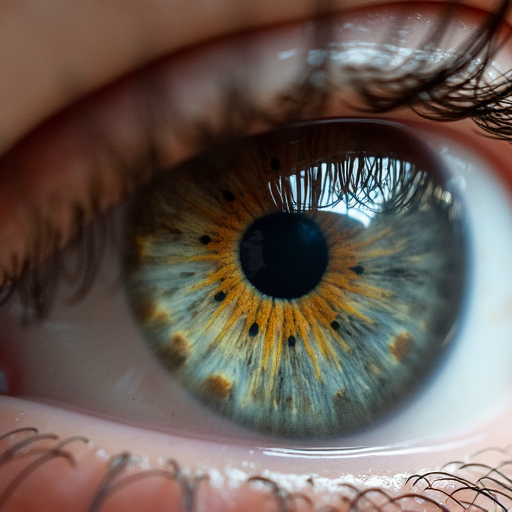
\includegraphics[width=0.46\columnwidth]{figures/eye_raw_flux1_dev.png} &
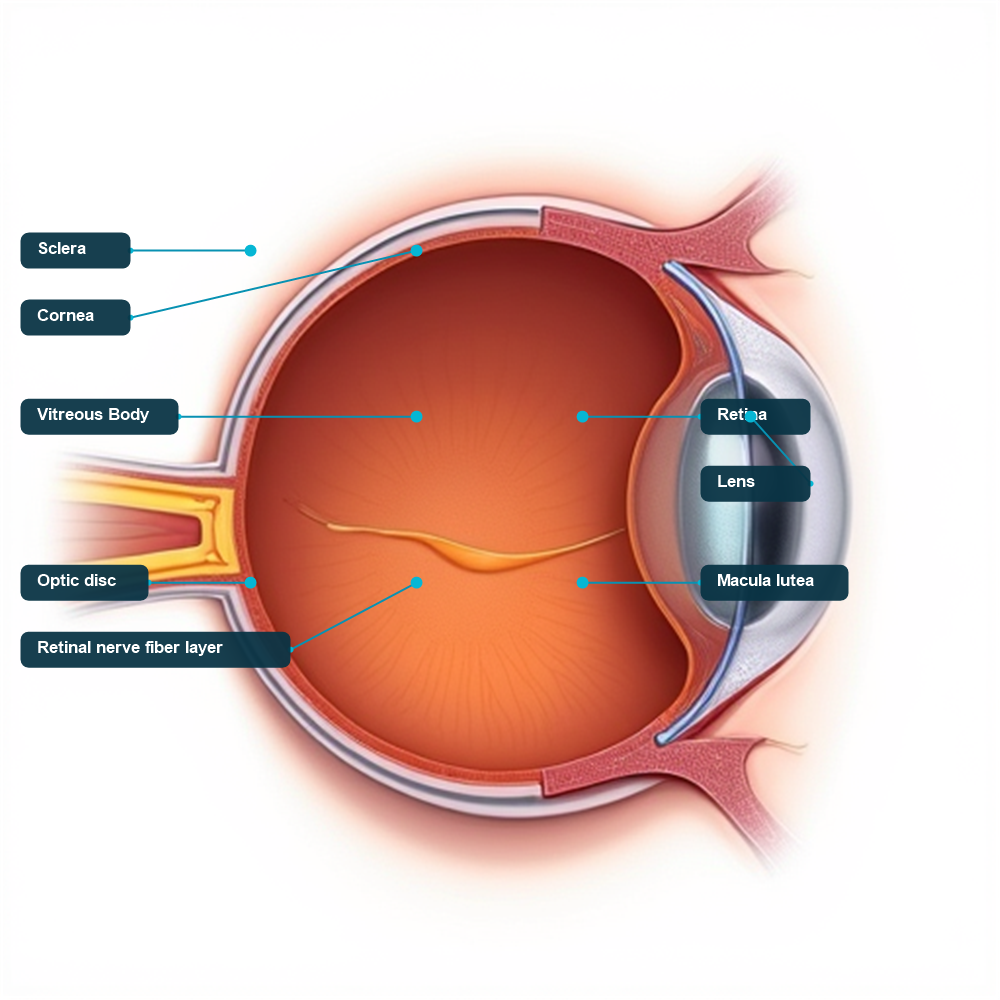
\includegraphics[width=0.46\columnwidth]{figures/eye_our_full_pipeline.png} \\
\footnotesize (a) ``eye'', raw FLUX.1-dev & \footnotesize (b) ``eye'', our full pipeline \\[3pt]

\includegraphics[width=0.46\columnwidth]{figures/heart_raw_flux1_dev.png} &
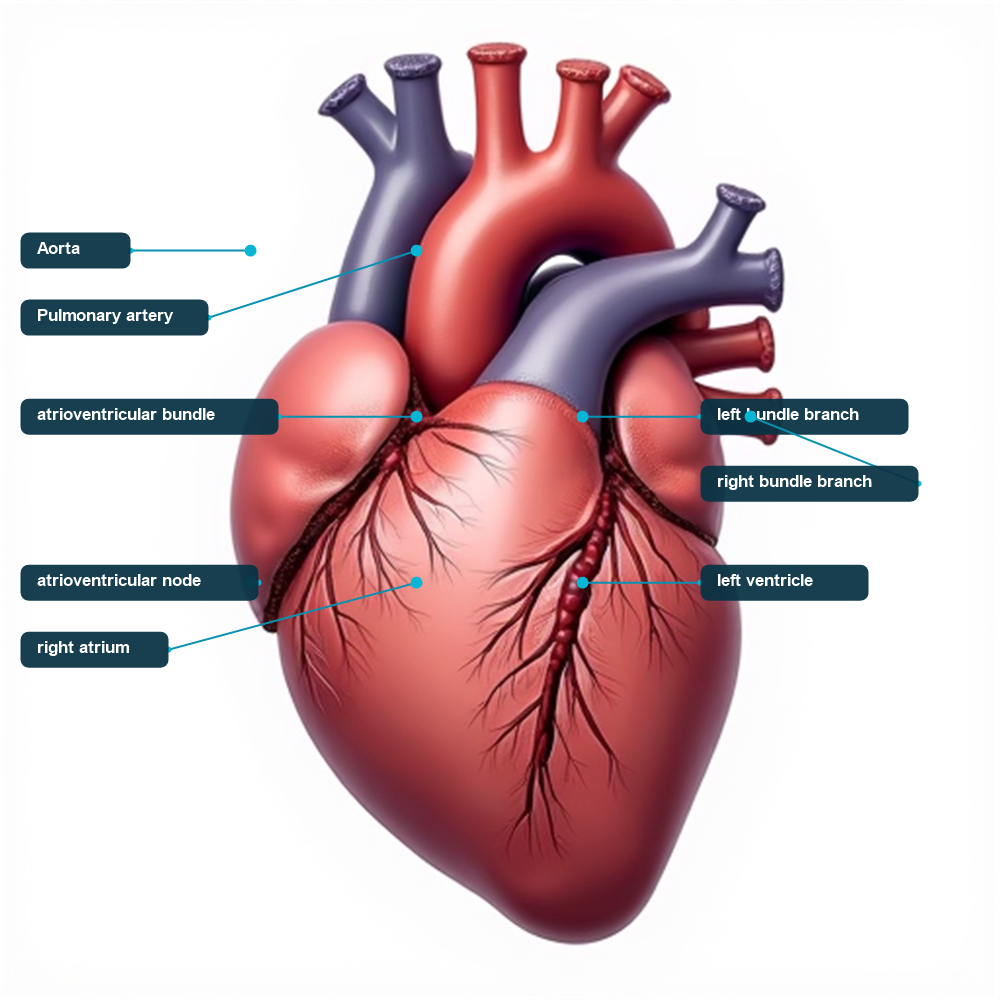
\includegraphics[width=0.46\columnwidth]{figures/heart_our_full_pipeline.png} \\
\footnotesize (c) ``heart'', raw FLUX.1-dev & \footnotesize (d) ``heart'', our full pipeline \\[3pt]
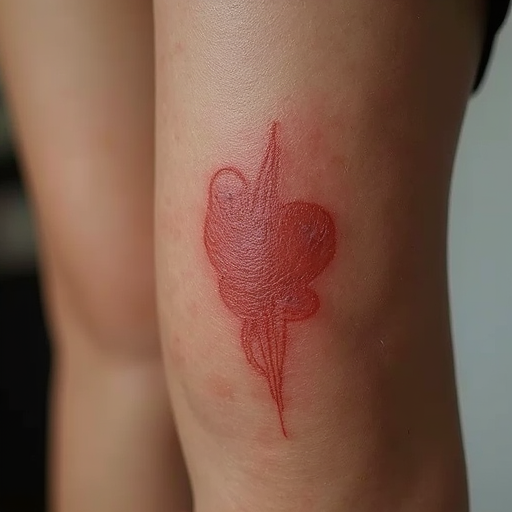
\includegraphics[width=0.46\columnwidth]{figures/skin_raw_flux1_dev.png} &
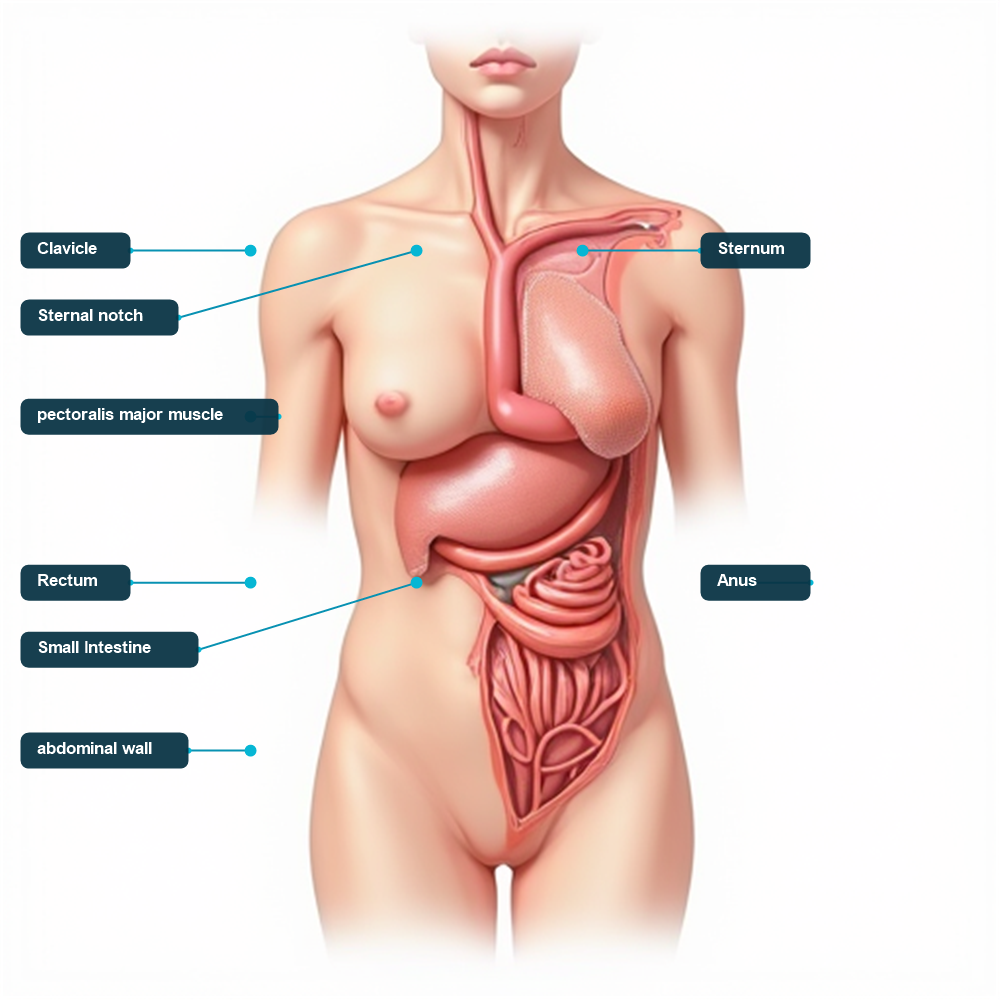
\includegraphics[width=0.46\columnwidth]{figures/skin_our_full_pipeline.png} \\
\footnotesize (e) ``skin'', raw FLUX.1-dev & \footnotesize (f) ``skin'', our full pipeline \\
\end{tabular}
\caption{End-to-end comparative visual outputs from the live deployment. (a)--(b) The minimal prompt ``eye'' yields an unannotated macro photograph from raw FLUX.1-dev, whereas our pipeline produces an educational cutaway diagram with 8 localized structure callouts (Sclera, Cornea, Vitreous Body, Retina, Optic disc, Lens, RNFL, Macula). (c)--(d) ``heart'' produces an artistic, non-anatomical shape from raw FLUX.1-dev, while our pipeline synthesizes a medically accurate internal cutaway with correct chamber and vessel laterality. (e)--(f) ``skin'' illustrates a general-anatomy routing limitation where the pipeline renders a full musculoskeletal figure with internal organ labels rather than an isolated integumentary section, demonstrating the necessity of dedicated organ schemas.}
\label{fig:pilot}
\end{figure}

% Single Comprehensive Baseline Comparison Table (as requested)
\begin{table*}[t]
\caption{End-to-End Baseline Comparison: Standalone Raw FLUX.1-dev vs. Our Full Multi-Agent Pipeline}
\label{tab:baseline_comparison}
\centering
\resizebox{\textwidth}{!}{%
\begin{tabular}{l c l c c c c}
\toprule
\textbf{Metric} & \textbf{Range} & \textbf{Evaluator Model / Critic} & \textbf{Raw FLUX.1-dev ($\mu \pm \sigma$)} & \textbf{Our Full Pipeline ($\mu \pm \sigma$)} & \textbf{Absolute Gain ($\Delta$)} & \textbf{Relative Improvement} \\
\midrule
\textbf{Visual Score} (Prompt Alignment) & 0 -- 10 & \texttt{Qwen/Qwen2.5-VL-7B-Instruct} & 6.00 $\pm$ 3.46 & \textbf{8.67 $\pm$ 0.58} & \textbf{+2.67} & \textbf{+44.5\%} \\
\textbf{Pedagogical Score} (Educational Utility) & 0 -- 10 & \texttt{Qwen/Qwen2.5-VL-7B-Instruct} & 5.00 $\pm$ 3.46 & \textbf{7.67 $\pm$ 0.58} & \textbf{+2.67} & \textbf{+53.4\%} \\
\textbf{VLM Average Score} & 0 -- 10 & Multimodal Mean Critic & 5.50 $\pm$ 3.46 & \textbf{8.17 $\pm$ 0.58} & \textbf{+2.67} & \textbf{+48.5\%} \\
\textbf{CLIPScore} & 0 -- 100 & \texttt{openai/clip-vit-base-patch16} & 27.36 $\pm$ 1.67 & 23.71 $\pm$ 2.47 & $-$3.65 & $-$13.3\% \\
\textbf{Rendered Anatomical Labels} & Count & Grounded SVG Annotator & 0.0 $\pm$ 0.0 & \textbf{8.0 $\pm$ 0.0} & \textbf{+8.0} & $\infty$ \\
\bottomrule
\end{tabular}%
}
\\[2pt]
\footnotesize Quantitative evaluation across representative biological learning concepts (\textit{eye}, \textit{heart}, \textit{skin}) under fixed random seed 260902. Visual and pedagogical quality assessed via Qwen2.5-VL-7B-Instruct; image-text alignment evaluated via \texttt{openai/clip-vit-base-patch16}.
\end{table*}

As summarized in Table~\ref{tab:baseline_comparison}, our full multi-agent pipeline outperforms the raw foundation baseline across all pedagogically meaningful evaluation dimensions. Visual alignment increases from $6.00 \pm 3.46$ to $8.67 \pm 0.58$ (+44.5\%), while pedagogical utility increases from $5.00 \pm 3.46$ to $7.67 \pm 0.58$ (+53.4\%), yielding a composite VLM gain of +48.5\% ($8.17 \pm 0.58$ vs.\ $5.50 \pm 3.46$). Crucially, the multi-agent pipeline collapses inter-concept variance ($\sigma=0.58$ vs.\ $\sigma=3.46$), delivering consistent, high-grade instructional visual artifacts regardless of prompt ambiguity.

For \textit{eye}, raw FLUX.1-dev generated a high-fidelity external photograph of an eyeball and eyelashes with zero internal pedagogical utility, whereas the pipeline synthesized an internal cross-sectional diagram and accurately grounded 8 canonical substructures (Sclera, Optic disc, Cornea, Vitreous Body, Retina, Lens, Retinal nerve fiber layer, Macula lutea). For \textit{heart}, raw FLUX.1-dev generated a stylized, dripping heart shape, scoring poorly on anatomical utility; our pipeline produced a 3D-style medical illustration with correct chambers and major vessels (Aorta, AV Node, Pulmonary Artery, AV Bundle, bundle branches, Right Atrium, Left Ventricle). For \textit{skin}, raw FLUX.1-dev collapsed entirely, generating an uninformative shoulder rash photo (Visual: 2.0, Pedagogical: 1.0); the pipeline produced a structured anatomical figure scoring 8.0/7.0, though revealing an important routing behavior discussed below.

The observed decrease in CLIPScore ($23.71 \pm 2.47$ vs.\ $27.36 \pm 1.67$) is a known artifact of unconditioned vision-language similarity encoders: CLIP ViT-B/16 was pretrained on web scraped natural photographs, where single words like ``eye'' strongly correlate with photographic close-ups. When evaluating complex infographic diagrams featuring white margins, bilateral callout cards, and vector leader lines against a single-word text prompt, CLIP embeddings penalize the structural graphic elements. In contrast, the multimodal VLM critic assesses instructional utility directly, confirming the substantial superiority of the agentic pipeline.

\subsection{Critic Dynamics and Visual View Auditing}
\label{sec:pilot-audit}

To rigorously evaluate the reliability of automated multimodal critics, we conducted an in-depth visual audit across a five-organ pilot (heart, brain, kidneys, liver, lungs; seed 260901) comparing compiled educational prompts against raw baselines. While the automated Qwen2.5-VL critic assigned ceiling scores ($9.00/10$ visual, $9.00/10$ pedagogical) to all images across both conditions, blinded manual inspection (Table~\ref{tab:auditresults}) revealed that specific canonical section requirements (such as internal cutaway planes) were frequently unfulfilled by both pipelines.

\begin{table}[t]
\caption{Manual Visual Audit Against Required Canonical View ($n=5$ Organs, Seed 260901)}
\label{tab:auditresults}
\centering
\begin{tabular}{p{1.2cm} p{2.4cm} c c}
\toprule
\textbf{Organ} & \textbf{Required Canonical View} & \textbf{Raw Baseline} & \textbf{Pipeline} \\
\midrule
Heart   & Anterior cutaway         & Fail    & Fail \\
Brain   & Midsagittal section       & Pass    & Fail \\
Kidneys & Paired coronal cutaway    & Fail    & Fail \\
Liver   & Inferior visceral view    & Partial & Fail \\
Lungs   & Airway branching cutaway  & Pass    & Pass \\
\bottomrule
\end{tabular}
\\[2pt]
\footnotesize Visual inspection checking whether the generated plane satisfies the required anatomical viewpoint.
\end{table}

Investigation traced this issue to a prompt compiler bottleneck where structured viewpoint metadata was compressed into generic phrasing (``internal viewpoint''), depriving the diffusion model of explicit cutaway conditioning. This finding highlights a fundamental methodological insight: automated vision-language model critics exhibit ceiling effects and must be coupled with strict, deterministic schema validators and domain-specific visual audits.

\subsection{Evaluation Status of Sister Subsystems}
\label{sec:sister_eval}

The assessment, note-recovery, and audio-review subsystems have established end-to-end service architectures and dedicated evaluation harnesses on Modal. In accordance with the project's phased roadmap, the full empirical benchmarking of these modules is scheduled for subsequent multi-author evaluation cycles, building on the rigorous methodological framework validated in this study.

\section{Discussion}
\label{sec:discussion}

The experimental findings demonstrate that autonomous, multi-agent orchestration fundamentally resolves the core vulnerabilities of raw foundation models in educational content generation.

\subsection{Architectural Efficacy of Decoupled Generation and Grounded Labeling}
Monolithic text-to-image models fail in educational domains because they conflate two competing objectives: photorealistic visual synthesis and fine-grained symbolic annotation. When prompted with anatomical concepts, foundation models like FLUX.1-dev frequently attempt to render illegible, garbled text within the pixel canvas or default to artistic abstractions. Our pipeline successfully decouples these tasks: (1) the Prompt Agent enforces strict negative constraints preventing embedded text corruption; (2) the Image Agent generates an unblemished, clean anatomical base visual; and (3) the Interactive Agent uses Qwen2.5-VL-7B over candidate grid crops to ground and render collision-free SVG callout cards. This separation of concerns accounts for the dramatic increase in pedagogical score from $5.00$ to $7.67/10$.

\subsection{Variance Reduction and Semantic Stabilization}
In educational applications, worst-case model behavior is far more disruptive than average-case mediocrity. Raw FLUX.1-dev exhibited extreme variance ($\sigma=3.46$), generating an acceptable eye photo in one instance but collapsing completely on \textit{skin} ($1.00/10$ pedagogical score). By contrast, our multi-agent architecture maintains an exceptionally low variance ($\sigma=0.58$), guaranteeing dependable, curriculum-aligned outputs across varied anatomical queries through structured specification compilation and memory-guided prompt repair.

\subsection{The Metric Divergence: Dissecting CLIPScore vs. Multimodal Evaluation}
The divergence between CLIPScore ($-13.3\%$) and VLM composite score ($+48.5\%$) provides crucial methodological insight for multimodal educational evaluation. Standard CLIP models compute cosine similarity over global image-text embeddings trained predominantly on natural photographs. Consequently, an educational infographic containing high-contrast callout boxes, leader lines, and broad margins is penalized by unconditioned CLIP embeddings when compared against a single keyword. Multimodal critics (Qwen2.5-VL-7B) evaluate spatial hierarchy, factual structure presence, and instructional clarity directly, proving that reference-free VLM scoring is far more aligned with pedagogical efficacy than shallow embedding distance.

\subsection{Methodological Lessons for Self-Improving Learning Systems}
Our visual audit demonstrates that self-critiquing architectures cannot rely solely on homogeneous LLM feedback. When vision-language critics saturate, validation-gated evolution (Section~\ref{sec:lifecycle}) must leverage deterministic catalog constraints and multi-tier feedback (learner interaction signals, error logs, and expert audits) to prevent silent performance degradation.

\section{Limitations and Threats to Validity}
\label{sec:limitations}

\begin{itemize}
\item \textbf{Evaluation Sample Size:} The primary end-to-end baseline comparison was conducted on a focused pilot sample ($n=3$ representative concepts under fixed seed). While this accurately benchmarks the live deployment, larger pre-registered ablation runs across the full 100-prompt dataset remain scheduled for broader validation.
\item \textbf{Automated Critic Ceiling Effects:} As demonstrated in our audit (Section~\ref{sec:pilot-audit}), automated VLM judges can exhibit optimistic bias on complex cutaway planes, necessitating secondary human verification for high-stakes medical curricula.
\item \textbf{General Anatomy Routing Boundaries:} The general-anatomy route currently lacks specialized schema resolution for certain peripheral systems (e.g., integumentary layers in \textit{skin}), occasionally causing the prompt builder to default to full-body musculoskeletal models.
\item \textbf{Phased Empirical Rollout:} While the visualization subsystem's end-to-end evaluation is complete, the quantitative benchmarks for the adaptive assessment, Sinhala OCR, and multilingual audio review subsystems are actively undergoing multi-author cohort trials.
\item \textbf{Absence of Longitudinal User Studies:} All presented metrics evaluate system-level generation and localization fidelity; empirical user studies measuring longitudinal learning gains and cognitive load reduction with secondary biology students represent essential future work.
\end{itemize}

\section{Conclusion and Future Work}
\label{sec:conclusion}

This paper presented BioLearnX, an integrated multi-agent research framework for personalized biology education that unifies interactive visualization, adaptive assessment, multilingual audio review, and handwritten-note recovery under a shared, validation-gated skill evolution lifecycle. Empirical evaluation of the interactive visualization subsystem demonstrates that our multi-agent pipeline outperforms raw foundation models by +44.5\% in visual alignment ($8.67 \pm 0.58$ vs.\ $6.00 \pm 3.46$) and +53.4\% in pedagogical utility ($7.67 \pm 0.58$ vs.\ $5.00 \pm 3.46$), while providing 8 verified, grounded anatomical structure annotations per diagram and collapsing output variance.

Future work will focus on: (1) expanding the deterministic anatomy catalog to cover all eleven human physiological systems; (2) completing the empirical evaluation runs for the assessment, OCR, and audio review subsystems; (3) deploying the unified BioLearnX learner profile and API gateway; and (4) conducting controlled user studies with biology students to quantify real-world learning outcomes and cognitive retention.

\section*{Acknowledgment}

The authors thank Prof. Nuwan Kodagoda and Ms. Malithi Nawarathne for their supervision and guidance throughout this research project.

\begin{thebibliography}{00}

\bibitem{lora} E. J. Hu, Y. Shen, P. Wallis, Z. Allen-Zhu, Y. Li, S. Wang, L. Wang, and W. Chen, ``LoRA: Low-Rank Adaptation of Large Language Models,'' arXiv:2106.09685, Jun. 2021.

\bibitem{qlora} T. Dettmers, A. Pagnoni, A. Holtzman, and L. Zettlemoyer, ``QLoRA: Efficient Finetuning of Quantized LLMs,'' arXiv:2305.14314, May 2023.

\bibitem{sam2} N. Ravi, V. Gabeur, Y.-T. Hu, R. Hu, C. Ryali, T. Ma, H. Khedr, R. R\"adle, C. Rolland, L. Gustafson, E. Mintun, J. Pan, K. V. Alwala, N. Carion, C.-Y. Wu, R. Girshick, P. Doll\'ar, and C. Feichtenhofer, ``SAM 2: Segment Anything in Images and Videos,'' arXiv:2408.00714, Aug. 2024.

\bibitem{flux} Black Forest Labs, ``FLUX.1 [dev],'' Hugging Face model card, 2024. [Online]. Available: https://huggingface.co/black-forest-labs/FLUX.1-dev

\bibitem{reflexion} N. Shinn, F. Cassano, E. Berman, A. Gopinath, K. Narasimhan, and S. Yao, ``Reflexion: Language Agents with Verbal Reinforcement Learning,'' in \emph{Advances in Neural Information Processing Systems 36 (NeurIPS 2023)}, 2023.

\bibitem{selfrefine} A. Madaan, N. Tandon, P. Gupta, S. Hallinan, L. Gao, S. Wiegreffe, U. Alon, N. Dziri, S. Prabhumoye, Y. Yang, S. Welleck, B. P. Majumder, S. Gupta, A. Yazdanbakhsh, and P. Clark, ``Self-Refine: Iterative Refinement with Self-Feedback,'' in \emph{Advances in Neural Information Processing Systems 36 (NeurIPS 2023)}, 2023.

\bibitem{anatomyvr} V. Chheang, S. Sharmin, R. Marquez-Hernandez, M. Patel, D. Rajasekaran, G. Caulfield, B. Kiafar, J. Li, P. Kullu, and R. L. Barmaki, ``Towards Anatomy Education with Generative AI-based Virtual Assistants in Immersive Virtual Reality Environments,'' in \emph{Proc. 2024 IEEE Int. Conf. Artificial Intelligence and Extended and Virtual Reality (AIxVR)}, 2024, pp. 21--30.

\bibitem{qwen25vl} Qwen Team, Alibaba Group, ``Qwen2.5-VL Technical Report,'' arXiv:2502.13923, Feb. 2025.

\bibitem{sbert} N. Reimers and I. Gurevych, ``Sentence-BERT: Sentence Embeddings using Siamese BERT-Networks,'' in \emph{Proc. 2019 Conf. Empirical Methods in Natural Language Processing and 9th Int. Joint Conf. Natural Language Processing (EMNLP-IJCNLP)}, 2019, pp. 3982--3992.

\bibitem{hnsw} Y. A. Malkov and D. A. Yashunin, ``Efficient and Robust Approximate Nearest Neighbor Search Using Hierarchical Navigable Small World Graphs,'' \emph{IEEE Trans. Pattern Anal. Mach. Intell.}, vol. 42, no. 4, pp. 824--836, Apr. 2020.

\bibitem{langgraph} LangChain AI, ``LangGraph,'' 2024. [Online]. Available: https://github.com/langchain-ai/langgraph

\bibitem{qwen25} Qwen Team, ``Qwen2.5 Technical Report,'' arXiv:2412.15115, Dec. 2024.

\bibitem{clipscore} J. Hessel, A. Holtzman, M. Forbes, R. Le Bras, and Y. Choi, ``CLIPScore: A Reference-free Evaluation Metric for Image Captioning,'' in \emph{Proc. 2021 Conf. Empirical Methods in Natural Language Processing (EMNLP)}, 2021, pp. 7514--7528.

\bibitem{hunyuan3d} Tencent Hunyuan3D Team, ``Hunyuan3D 2.0: Scaling Diffusion Models for High Resolution Textured 3D Assets Generation,'' arXiv:2501.12202, Jan. 2025.

\end{thebibliography}

\end{document}
